\begin{figure}
    	\centering
    	\begin{minipage}{1\textwidth}
    		\centering
    		\begin{minipage}{0.45\textwidth}
    			\centering
    			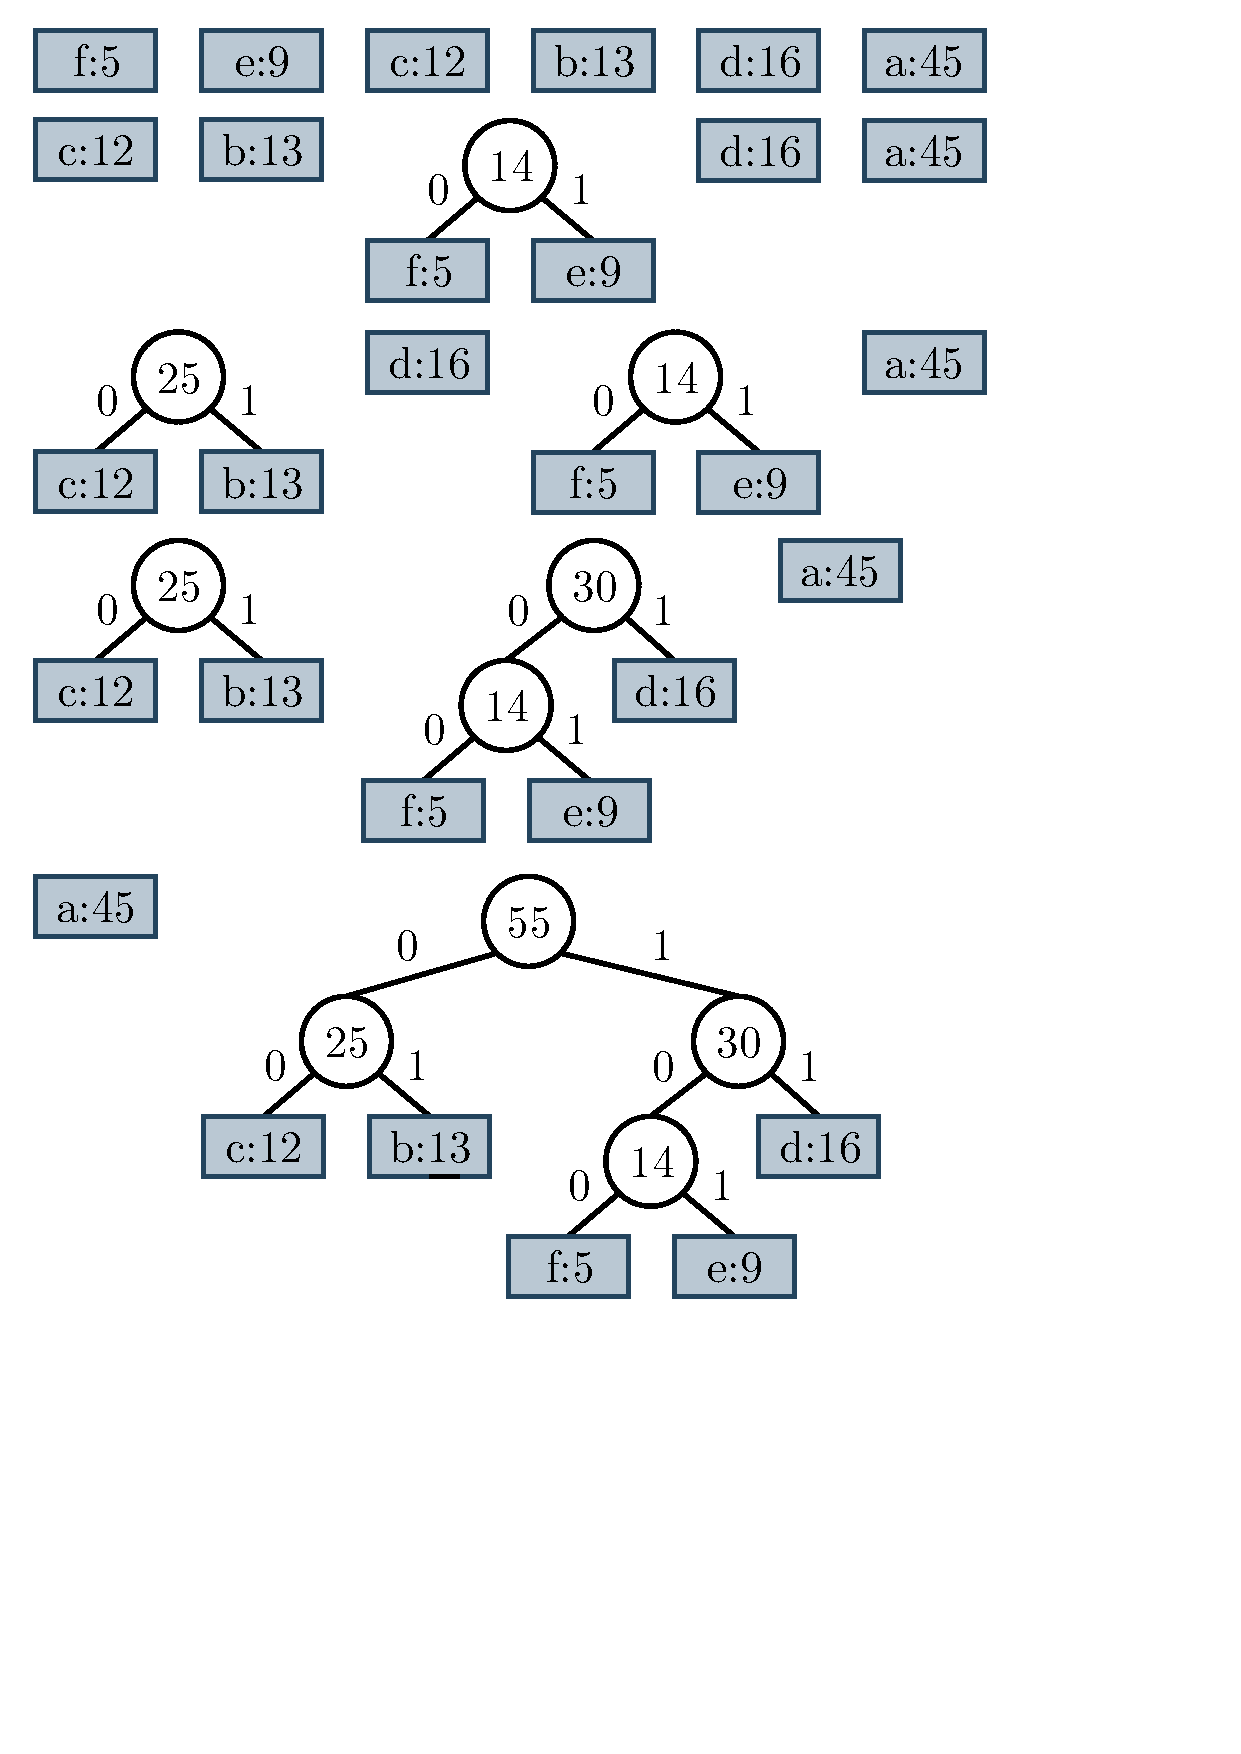
\includegraphics[scale=.45, clip, trim=16 790 120 10]{img/graphs-huffman2.pdf}
    			
    			(a)
    		\end{minipage}
    		\begin{minipage}{0.45\textwidth}
    			\centering
    			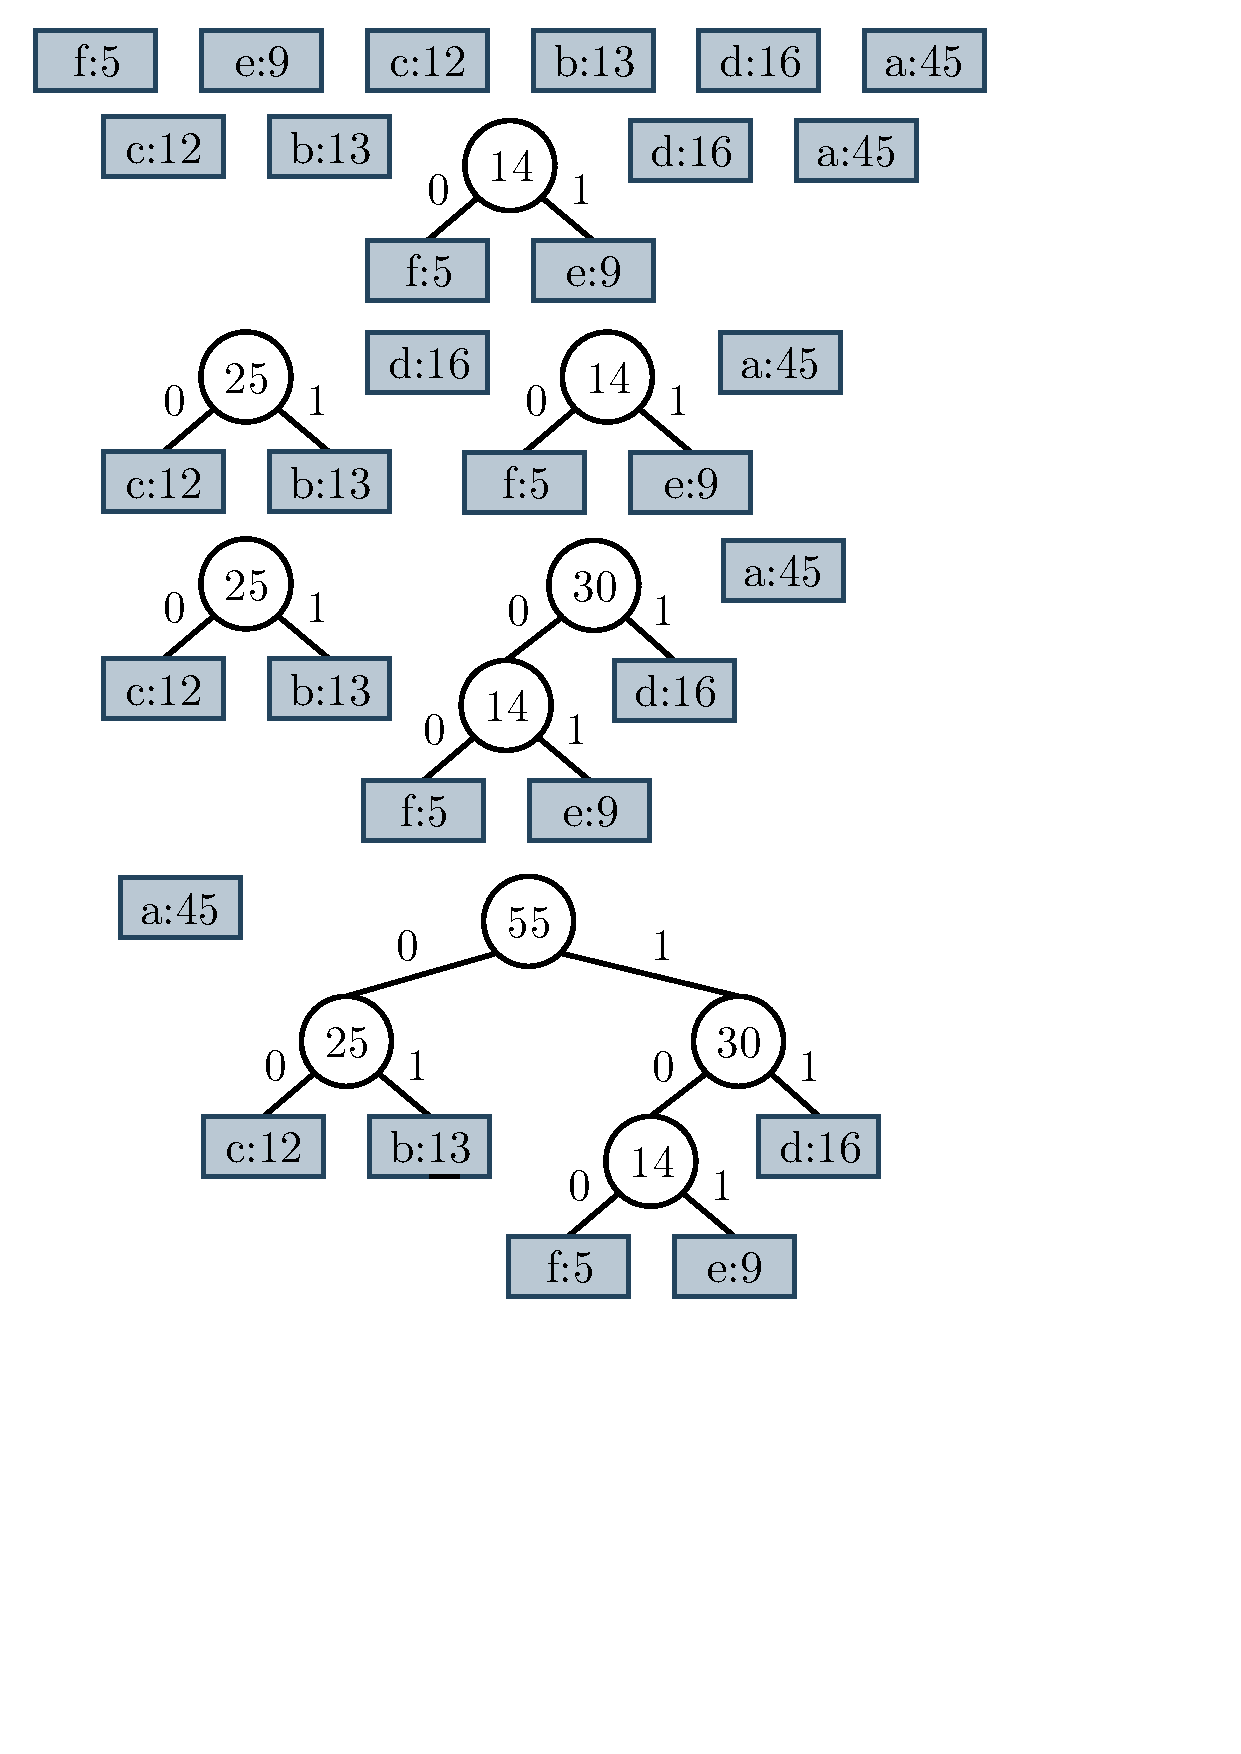
\includegraphics[scale=.45, clip, trim=40 690 150 50]{img/graphs-huffman21.pdf}

    			(b)
    		\end{minipage}  		
    	\end{minipage}
    	
    	\begin{minipage}{1\textwidth}
    		\centering
    		\begin{minipage}{0.45\textwidth}
    			\centering
    			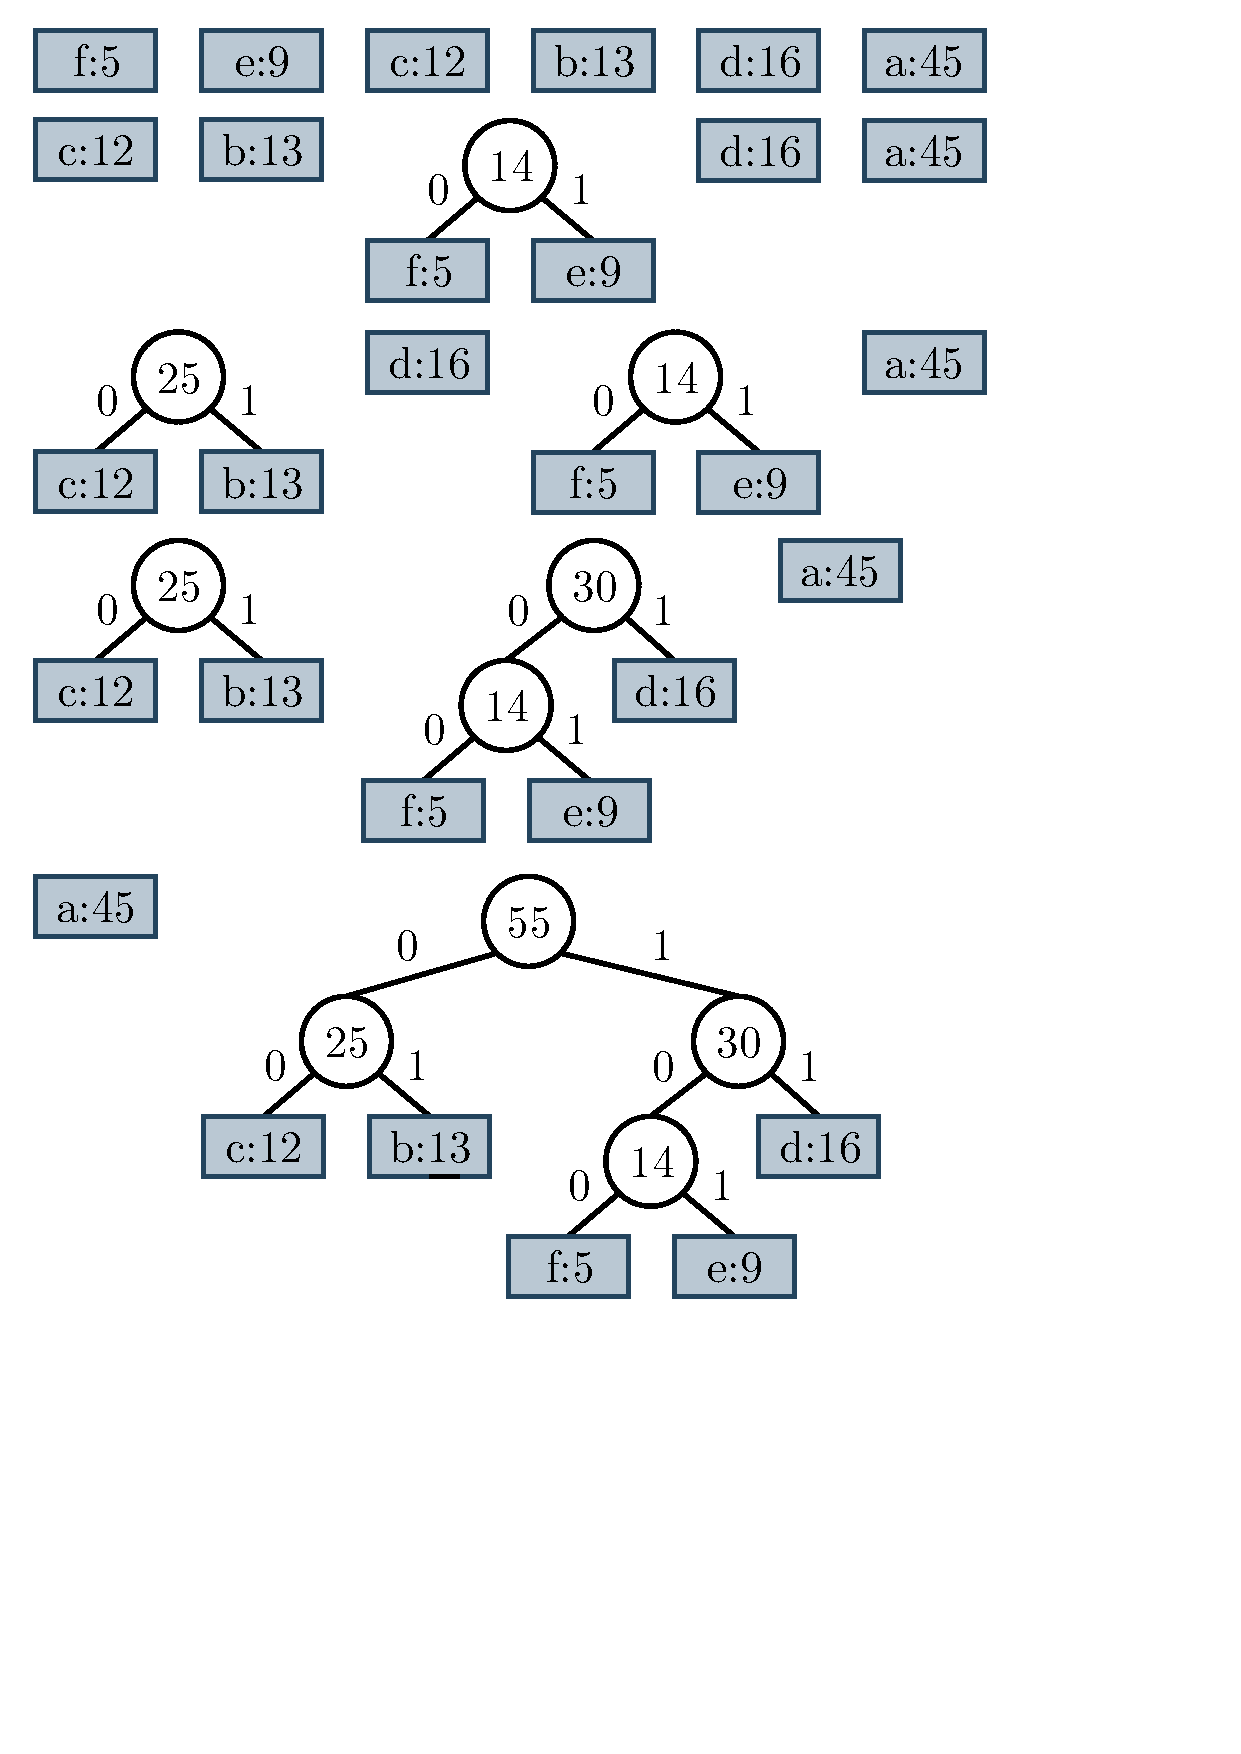
\includegraphics[scale=.4, clip, trim=10 590 120 150]{img/graphs-huffman2.pdf}
    			
    			(c)
    		\end{minipage}
    		\begin{minipage}{0.45\textwidth}
    			\centering
    			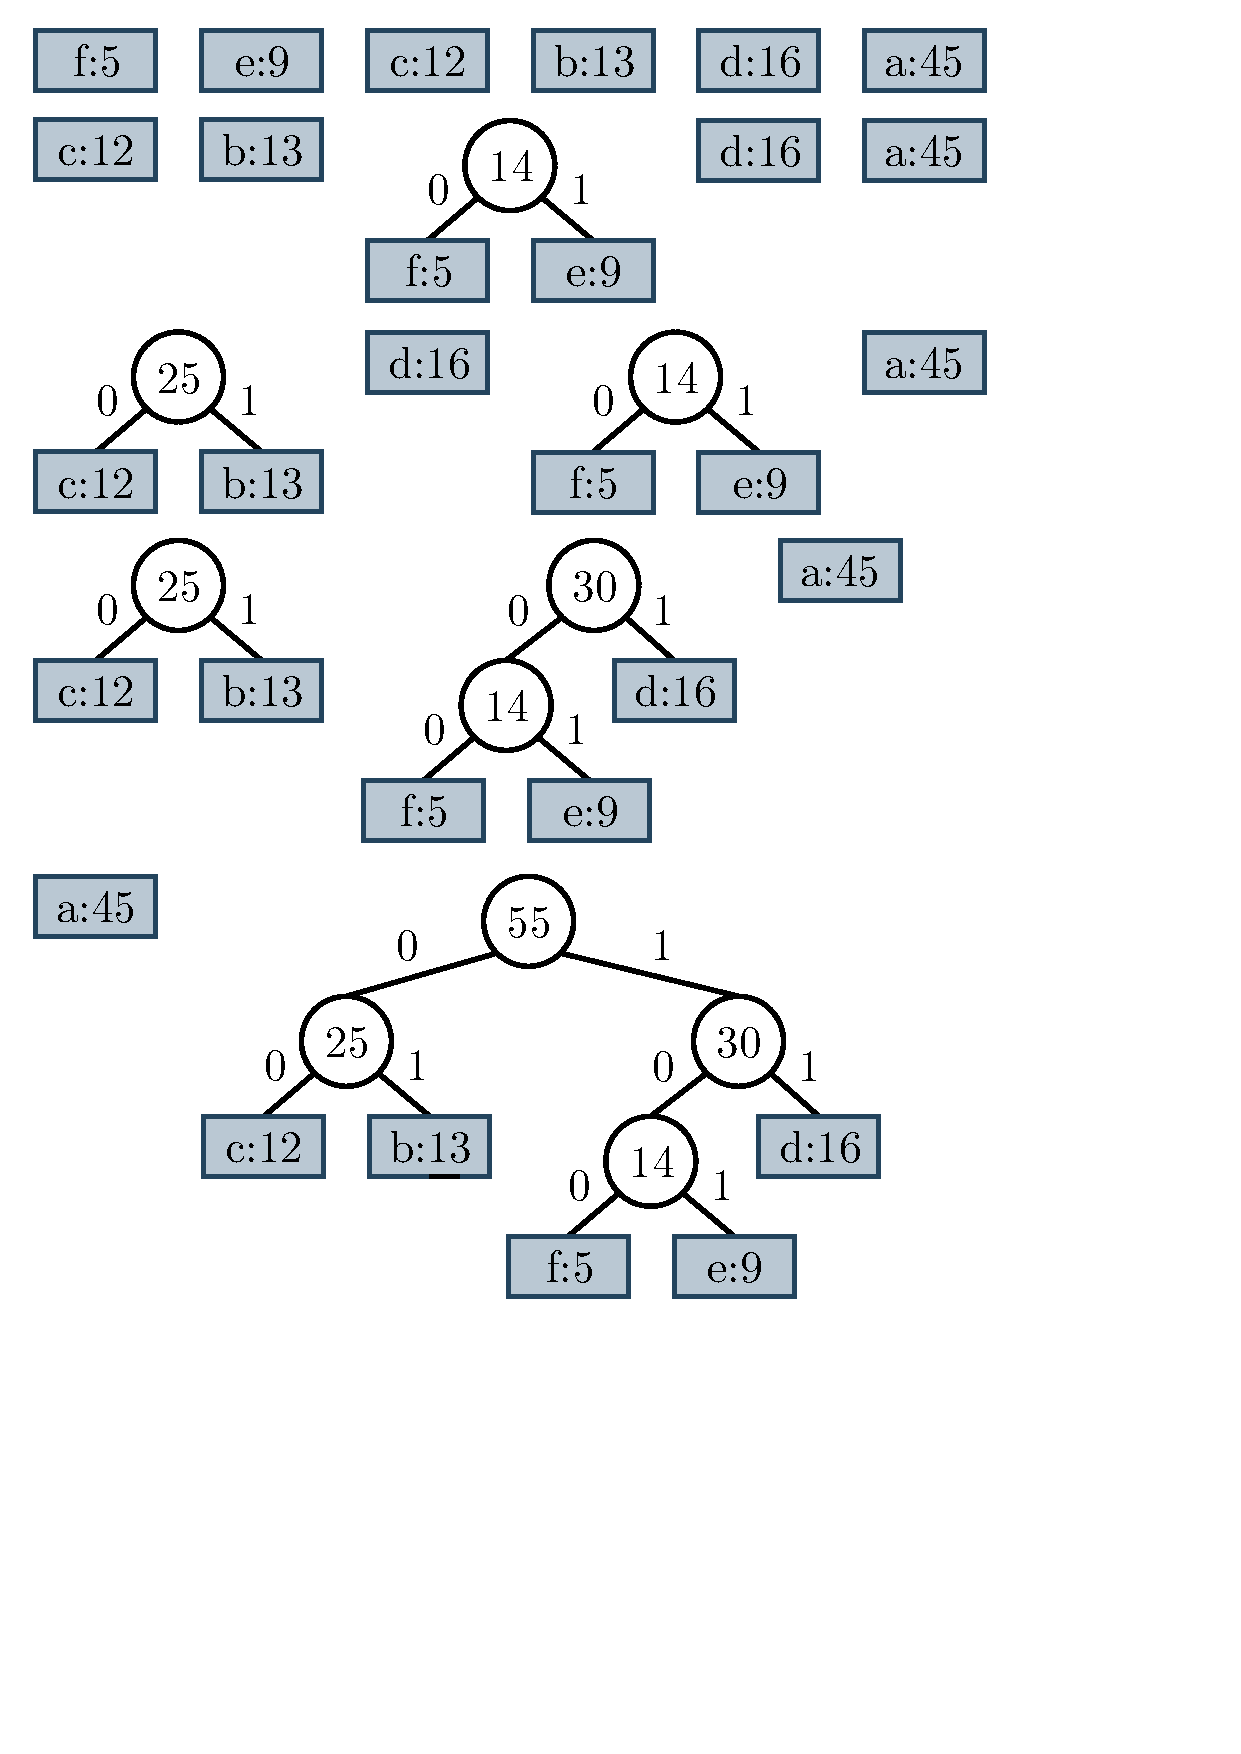
\includegraphics[scale=.4, clip, trim=10 430 160 250]{img/graphs-huffman2.pdf}
    			
    			(d)
    		\end{minipage}  
    	\end{minipage}
    	
    \begin{minipage}{1\textwidth}
    		\centering
    		\begin{minipage}{0.45\textwidth}
    			\centering
    			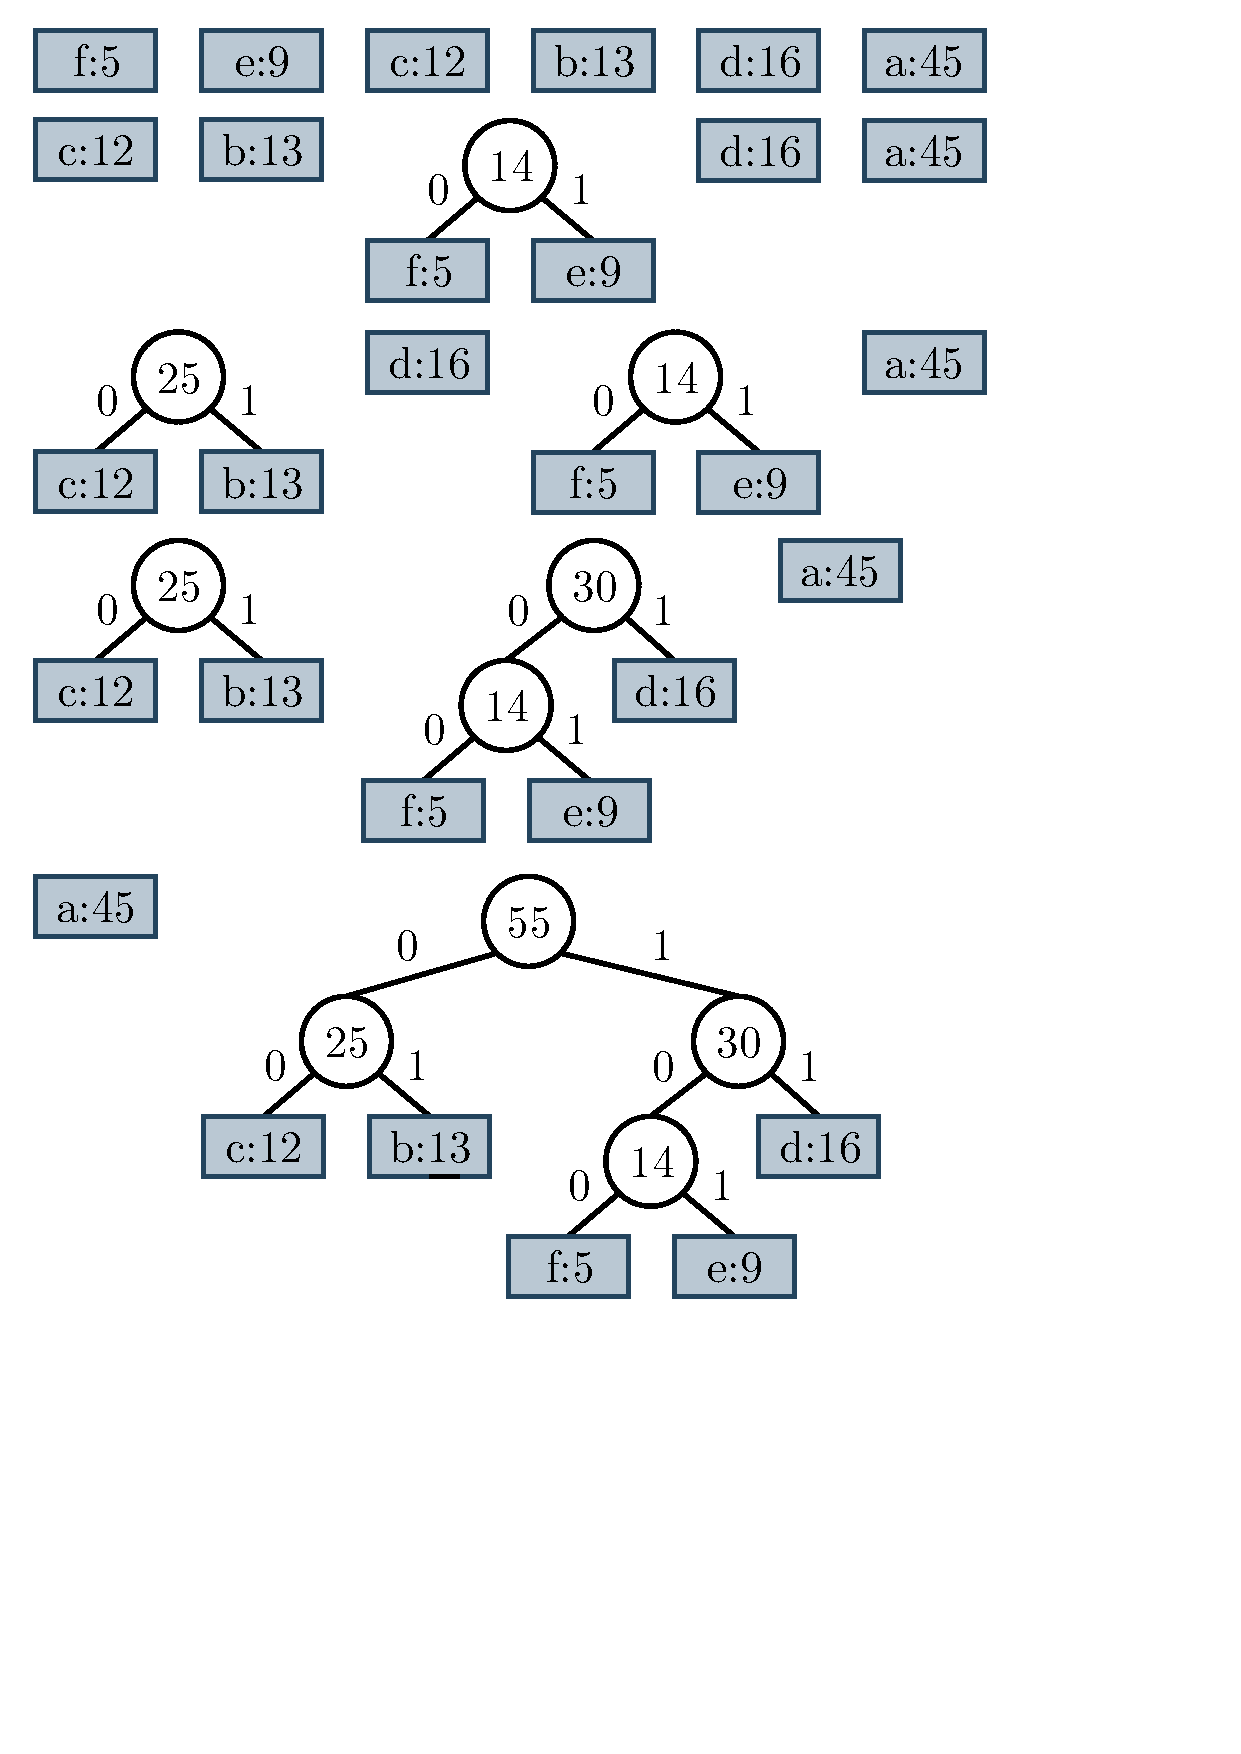
\includegraphics[scale=.4, clip, trim=10 210 170 410]{img/graphs-huffman2.pdf}
    			
    			(e)
    		\end{minipage}
    		\begin{minipage}{0.45\textwidth}
    			\centering
    			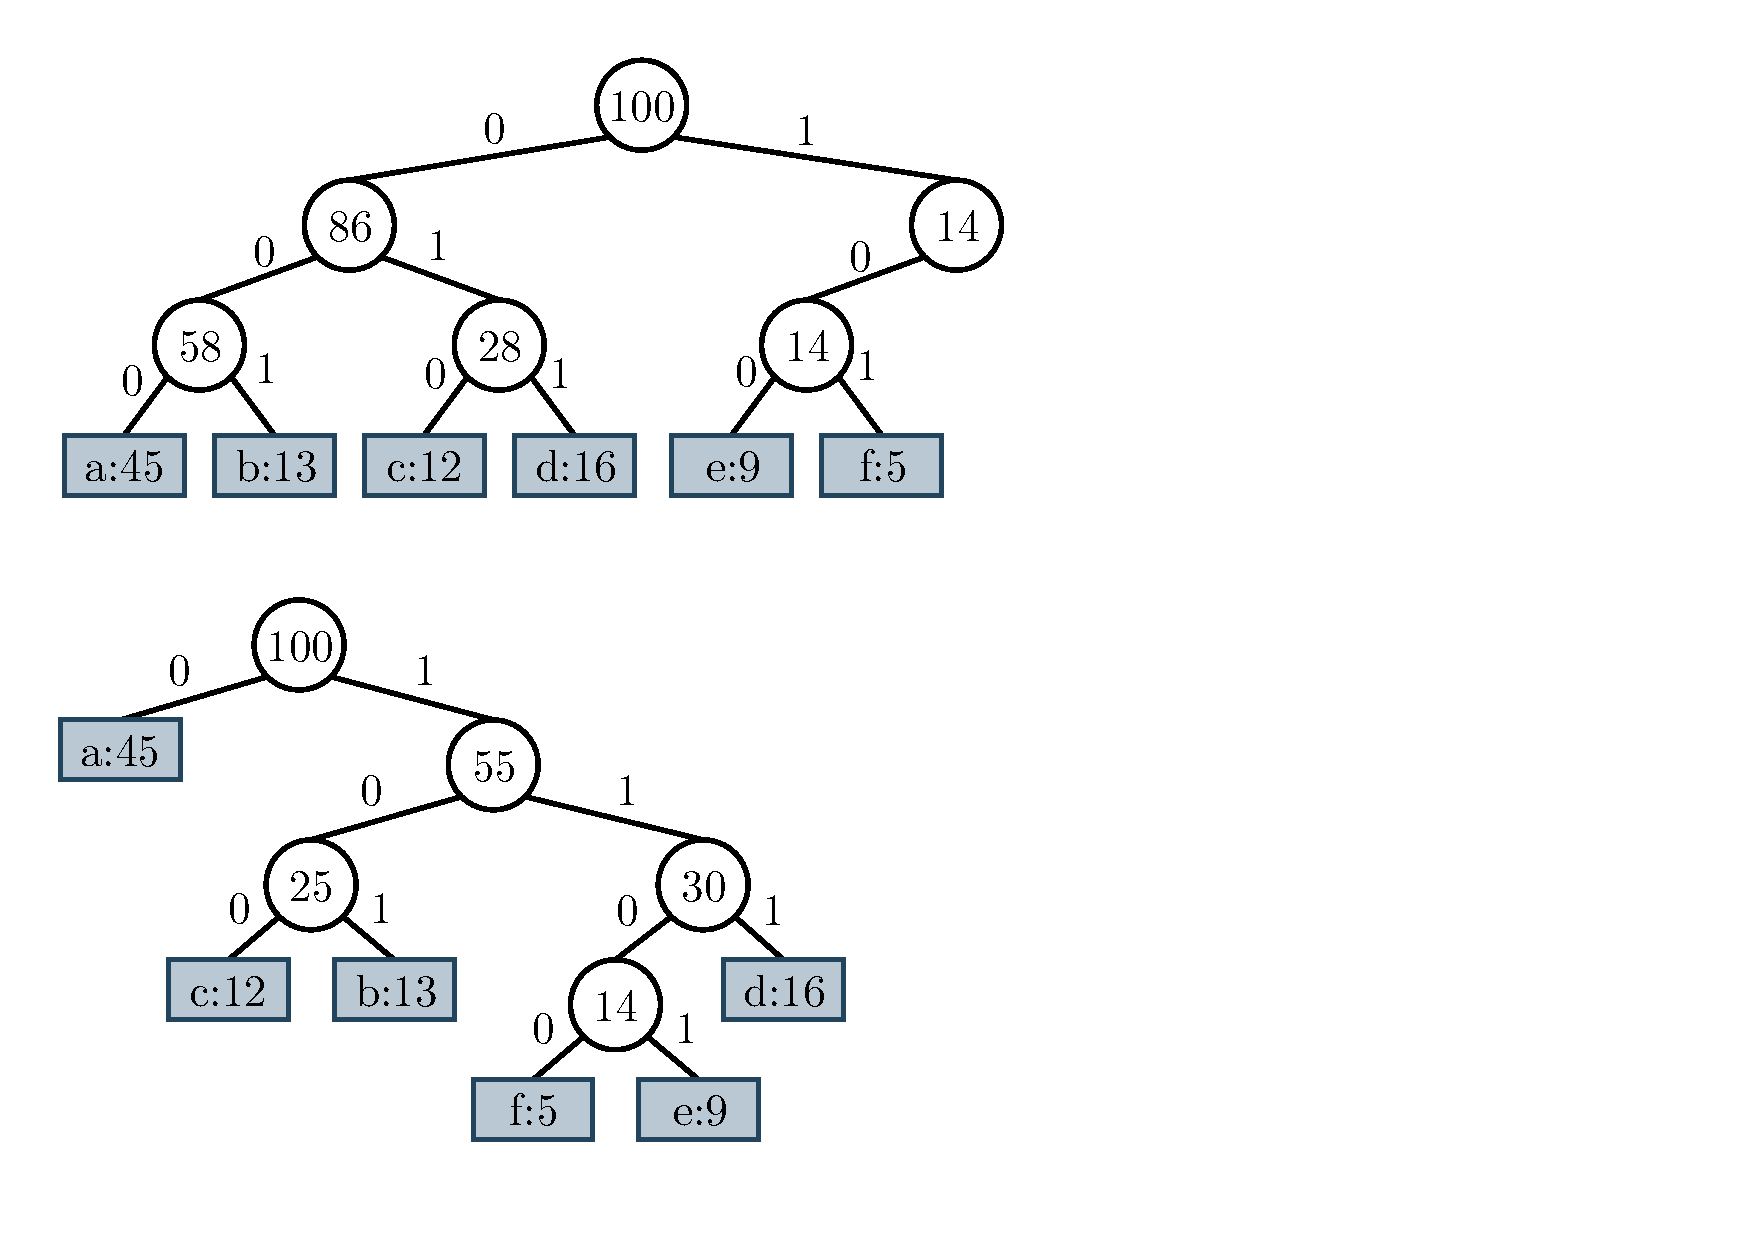
\includegraphics[scale=.4, clip, trim=20 40 430 280 ]{img/graphs-fixVarTrees.pdf}

    			(f)
    		\end{minipage}  
    	\end{minipage}
    	
    	 
    \caption{Etapas de construcción para codificación Huffman, para secuencia $C$ ejemplo.}% (a) Los 6 nodos hojas iniciales. (b) Primera unión. (c) Segunda unión. (d) Tercera unión. (e) Cuarta unión. (f) Quinta y última unión.}
    \label{fig:huffman2}
\end{figure}
